\documentclass[11pt, letterpaper]{article}
\usepackage[utf8]{inputenc}
\usepackage[letterpaper, margin=0.5in]{geometry}
\usepackage{amsmath}
\usepackage{amssymb}
\usepackage{amsthm}
\usepackage{graphicx}
\usepackage{listings}
\usepackage[font=scriptsize]{caption}
\usepackage{subcaption}
\usepackage{xcolor}

\newtheorem{lemma}{Lemma}
\newcommand{\indep}{\perp \!\!\! \perp}

\definecolor{codegreen}{rgb}{0,0.6,0}
\definecolor{codegray}{rgb}{0.5,0.5,0.5}
\definecolor{codepurple}{rgb}{0.58,0,0.82}
\definecolor{backcolour}{rgb}{0.95,0.95,0.92}

\lstdefinestyle{mystyle}{
    backgroundcolor=\color{backcolour},   
    commentstyle=\color{codegreen},
    keywordstyle=\color{magenta},
    numberstyle=\tiny\color{codegray},
    stringstyle=\color{codepurple},
    basicstyle=\ttfamily\footnotesize,
    breakatwhitespace=false,
    texcl=true,
    mathescape=true,
    breaklines=true,                 
    captionpos=b,                    
    keepspaces=true,                 
    numbers=left,                    
    numbersep=5pt,                  
    showspaces=false,                
    showstringspaces=false,
    showtabs=false,                  
    tabsize=2
}

\lstset{style=mystyle}
\graphicspath{ {../statics/} }
\captionsetup{justification=raggedright, singlelinecheck=false}

\author{Ryan Tang}
\title{STA 532 HW 6}
\date{March 5th 2023}

\begin{document}
\maketitle

\section{Ex 3-1}
\paragraph{(a)}
Generally, assuming the $H_o$ is true, the p-value follows a uniform distribution. It is shown below. Let $F(.)$ be the cdf function of distribution and $T(X) = t$ be the test statistics. Our binomial cases simplify the test statistics to $T(X) = x_{obs}$.
\begin{align*}
    p &= P(T(X) \ge t | H_o) \\
        &= 1 - P(T(X) < t | H_o) \\
        &= 1 - F_{H_o}(t) \\
    F_{H_o}(t) &= 1 - p \\
    p_{H_o}(p) &= \frac{\partial}{\partial t} F_{H_o}(t) = 1 \thicksim U(0, 1)
\end{align*}

\paragraph{(b)}
It has become obvious due to the proof of (a) that the test rule $\delta(x) = $ "reject $H_o$ if $p < \alpha$, $\alpha \in (0, 1)$". Because assuming the $H_o$ is true, the chance we get it wrong by following the rule $delta(x)$ is $\alpha$ asymptotically, which is the Type I error.

\paragraph{(c)}
Now, we have the data $n=500, x = 300$ under our binomial opinion poll case. Assuming we reject the $H_o$ at $\alpha = 0.00001$, the corresponding $\beta$ ratio can be found by first finding the critical value $c$.
\begin{align*}
    X &\thicksim Binom(n=500, p=\phi) \\
    \alpha &= 0.00001 = P(X \ge x_{obs} | \phi = 0.5) \\
    c &= F^{-1}(q=0.00001, n=500, \phi=0.5) = 298 \\
    \beta &= P(X \le c | \phi = 0.6) \approx 0.44
\end{align*}

\paragraph{(d)}
Here we fix the test rule from (c), $\delta(x) = $ "reject $H_o$ if $p < \alpha, \alpha=0.00001, \beta=0.44$". Then, we can compare it with a different test rule under the same binomial assumption, $\delta'(x) = $ "reject $H_o$ if $p < \alpha, \alpha=0.05, \beta=0.002$". Rejecting or accepting either rule gives an entirely different interpretation. Especially the former is much more conservative than the latter. Hence, due to conservatism, the change of Type II error is inflated at the pre-determined $H_o$ and $H_1$. 


\section{Ex 3-3}
\paragraph{(d)}
The conditional p-value $p = P(T(X) \ge t|H_o)$ should follow a uniform distribution because the $H_o$ and the corresponding test statistics are sufficient, which follows the same argument in the proof from 3.1(a). The maximum operator in Fisher's p-value drops because of the conditional. However, the complication comes in due to the composition and unconditional p-value "$\mathop{\max}_{P\in \mathcal{P}_o} P(T(X) \ge t)$", which can be multi-modal weirdly shaped.

\newpage
\section{Ex 3-4}
We like to experiment to see if there is a trend on the tropical cyclone annual count dataset, $X =(X_1, X_2, \dots, X_n)$. Under Fisher's framework, we have the null hypothesis $H_o: X_i \thicksim_{iid} \text{Poisson}(\alpha)$. And the test statistics, $T=\frac{W}{\bar{X}+1/n}, W=\frac{1}{n(n+1)}\sum_j^n jX_j$. The sufficient statistics for the experiment are also collected, $n=100, W = 4.69, \bar{X}=8.77, T=0.534$. Hence, Fisher's p-value equals $\max_{\alpha>0} P(T\ge 0.534|\alpha)$.

\paragraph{(a)}
First, since it maximizes over all possible $\alpha$, we run a Monte Carlo to estimate the p-value, and the distribution of p-values against various $\alpha$ is plotted below. We can see that Fisher's p-value is maximized when $\alpha \approx 0.162, p = 0.172$. This is the p-value that would be reported under the framework.

\begin{figure*}[!h]
  \centering
  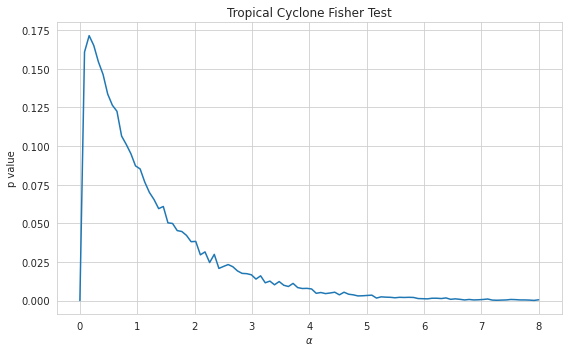
\includegraphics[width=0.6\textwidth]{hw6-1.png}
  \captionsetup{justification=centering}
  % \caption{}
  % \label{fig:sufficient-logl}
\end{figure*}

\section{Ex 3-5}


\end{document}